\subsubsection{Attitude Controller Simulation}
In the following section the final design of the attitude controller is given. Hence the final pole locations from the state feedback and the observer are provided. The final response, step response and observer estimation of the attitude controller can therefore be analysed and discussed. To be able to discussed the final result and illustrate the iteration process which has been used to find the final pole locations, the state feedback and observer are changed. Thus it is possible to yield reasoning for why the final design of the attitude controller is as it is.

A short description for the following three figures, \autoref{fig:ssFinalEq}, \autoref{fig:ssObsFinal} and \autoref{fig:ssFinalStep}, which is the final system response, step response and the estimation is given. The weighted matrices, $\vec{Q}$ and $\vec{R}$, utilized for the final attitude controller can be seen in \autoref{app:matricesSS}.

In \autoref{fig:ssFinalEq} a simulated angle response of the final attitude controller is shown. Initial conditions at time zero are given to the three angles. These are set to $0.2$ radians for the pitch, $-0.3$ for the roll and $-0.2$ for the yaw. The reference which the three angles is set to converge to is zero. \\ It can be seen from the figure that it approximately takes $2.5$ seconds for the pitch and roll to settle at zero, where it only takes approximately $1.4$-$1.5$ for the yaw.

\begin{figure}[H]
	\centering
	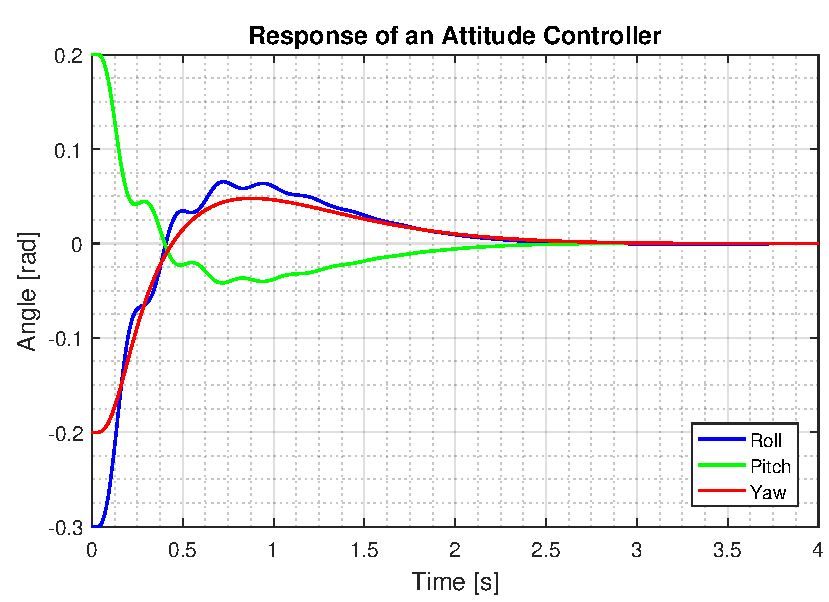
\includegraphics[scale=0.8]{figures/ssFinalEq.pdf}
	\caption{System response of the attitude controller, with initial conditions of $0.2$ radians for the pitch, $-0.3$ radians for the roll and $-0.2$ radians for the yaw. The weighted matrices, $\vec{Q}$ and $\vec{R}$, which are utilized for the final design can be seen in \autoref{app:matricesSS}.}
	\label{fig:ssFinalEq}
\end{figure}

In \autoref{fig:ssObsFinal} the estimation for the angular velocity in roll, pitch and yaw generated by the observer is shown. The simulation is related with the angle response shown in \autoref{fig:ssFinalEq}, as these are the angular velocity generated by the angle response with these initial conditions. To be able to evaluate the observers estimation, the red line, the actual angular velocity in roll, pitch and yaw is illustrated as well, the blue line. \\
A few differences between the actual velocity and the estimated can be seen. The first estimation generated by the observer, the high increase in the beginning is due to the initial conditions for the angles. 

\begin{figure}[H]
	\centering
	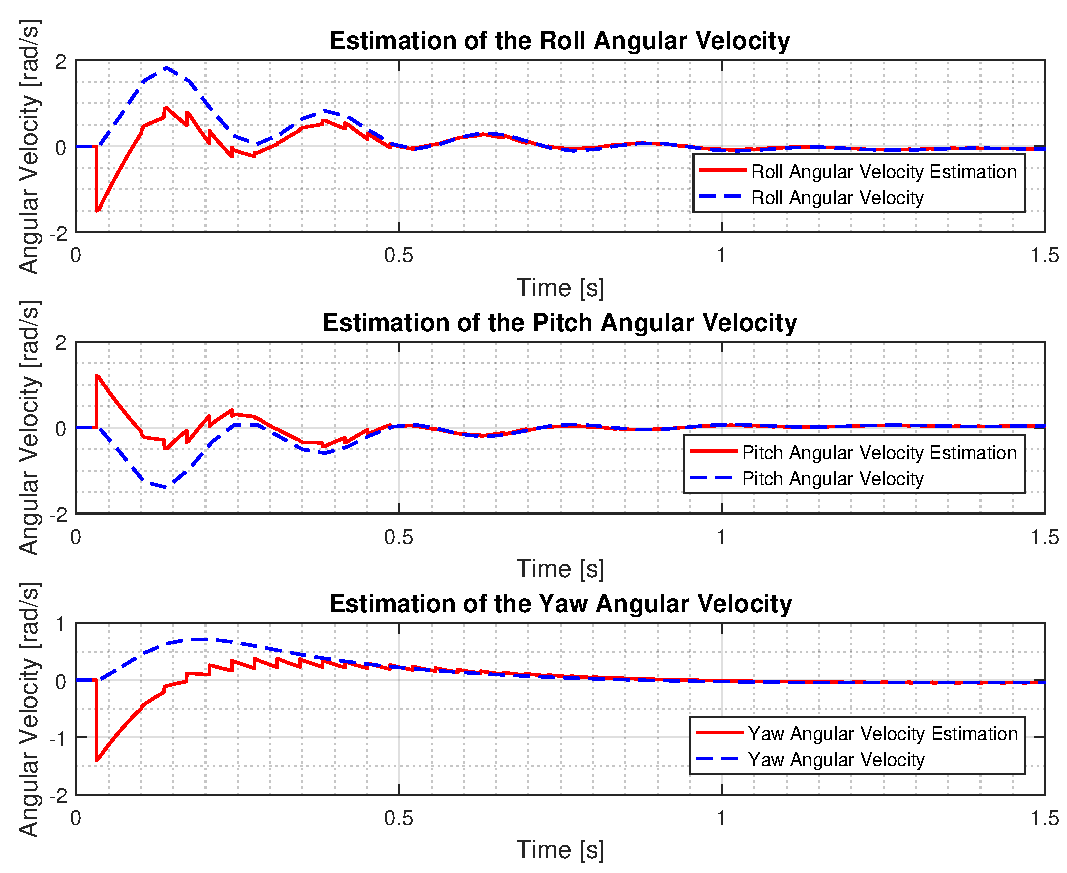
\includegraphics[scale=0.7]{figures/ssObsFinal.pdf}
	\caption{\autoref{app:matricesSS}.}
	\label{fig:ssObsFinal}
\end{figure}

why are there spikes / delay. Sampling frequency 35 ms.

Final step response:

\begin{figure}[H]
	\centering
	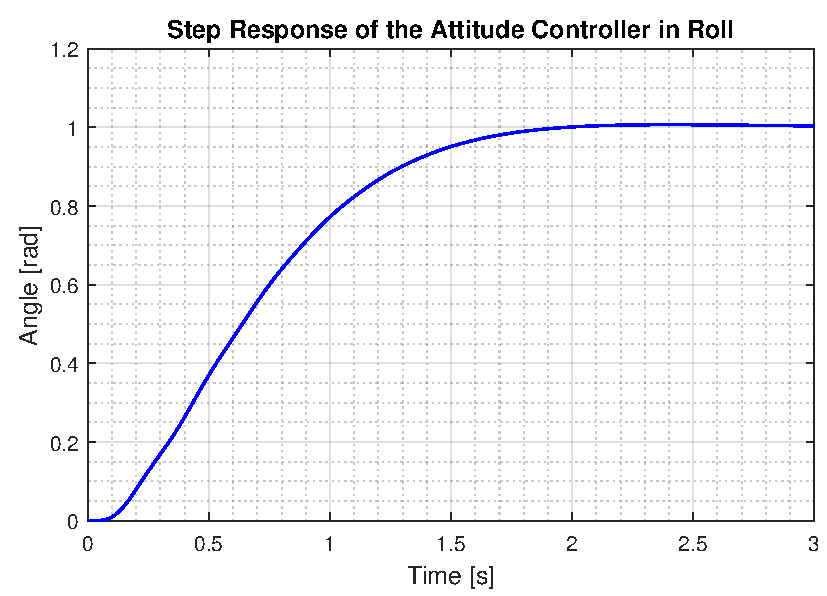
\includegraphics[scale=0.8]{figures/ssFinalStep.pdf}
	\caption{\autoref{app:matricesSS}.}
	\label{fig:ssFinalStep}
\end{figure}

Final Observer Estimator:

steady state margin 5 percent

rise time

setling time

overshoot

The yaw because the reference is always zero, as we do not want to track the yaw.


Higher F gain:

\begin{figure}[H]
	\centering
	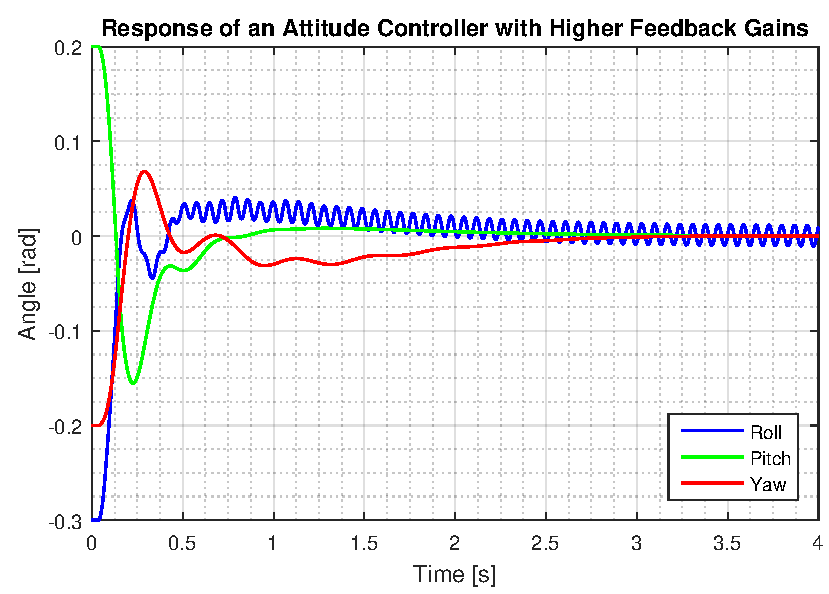
\includegraphics[scale=1]{figures/ssEqBad.pdf}
	\caption{\autoref{app:matricesSS}.}
	\label{fig:TranslationalControlDiagram}
\end{figure}

High Estimation L:

\begin{figure}[H]
	\centering
	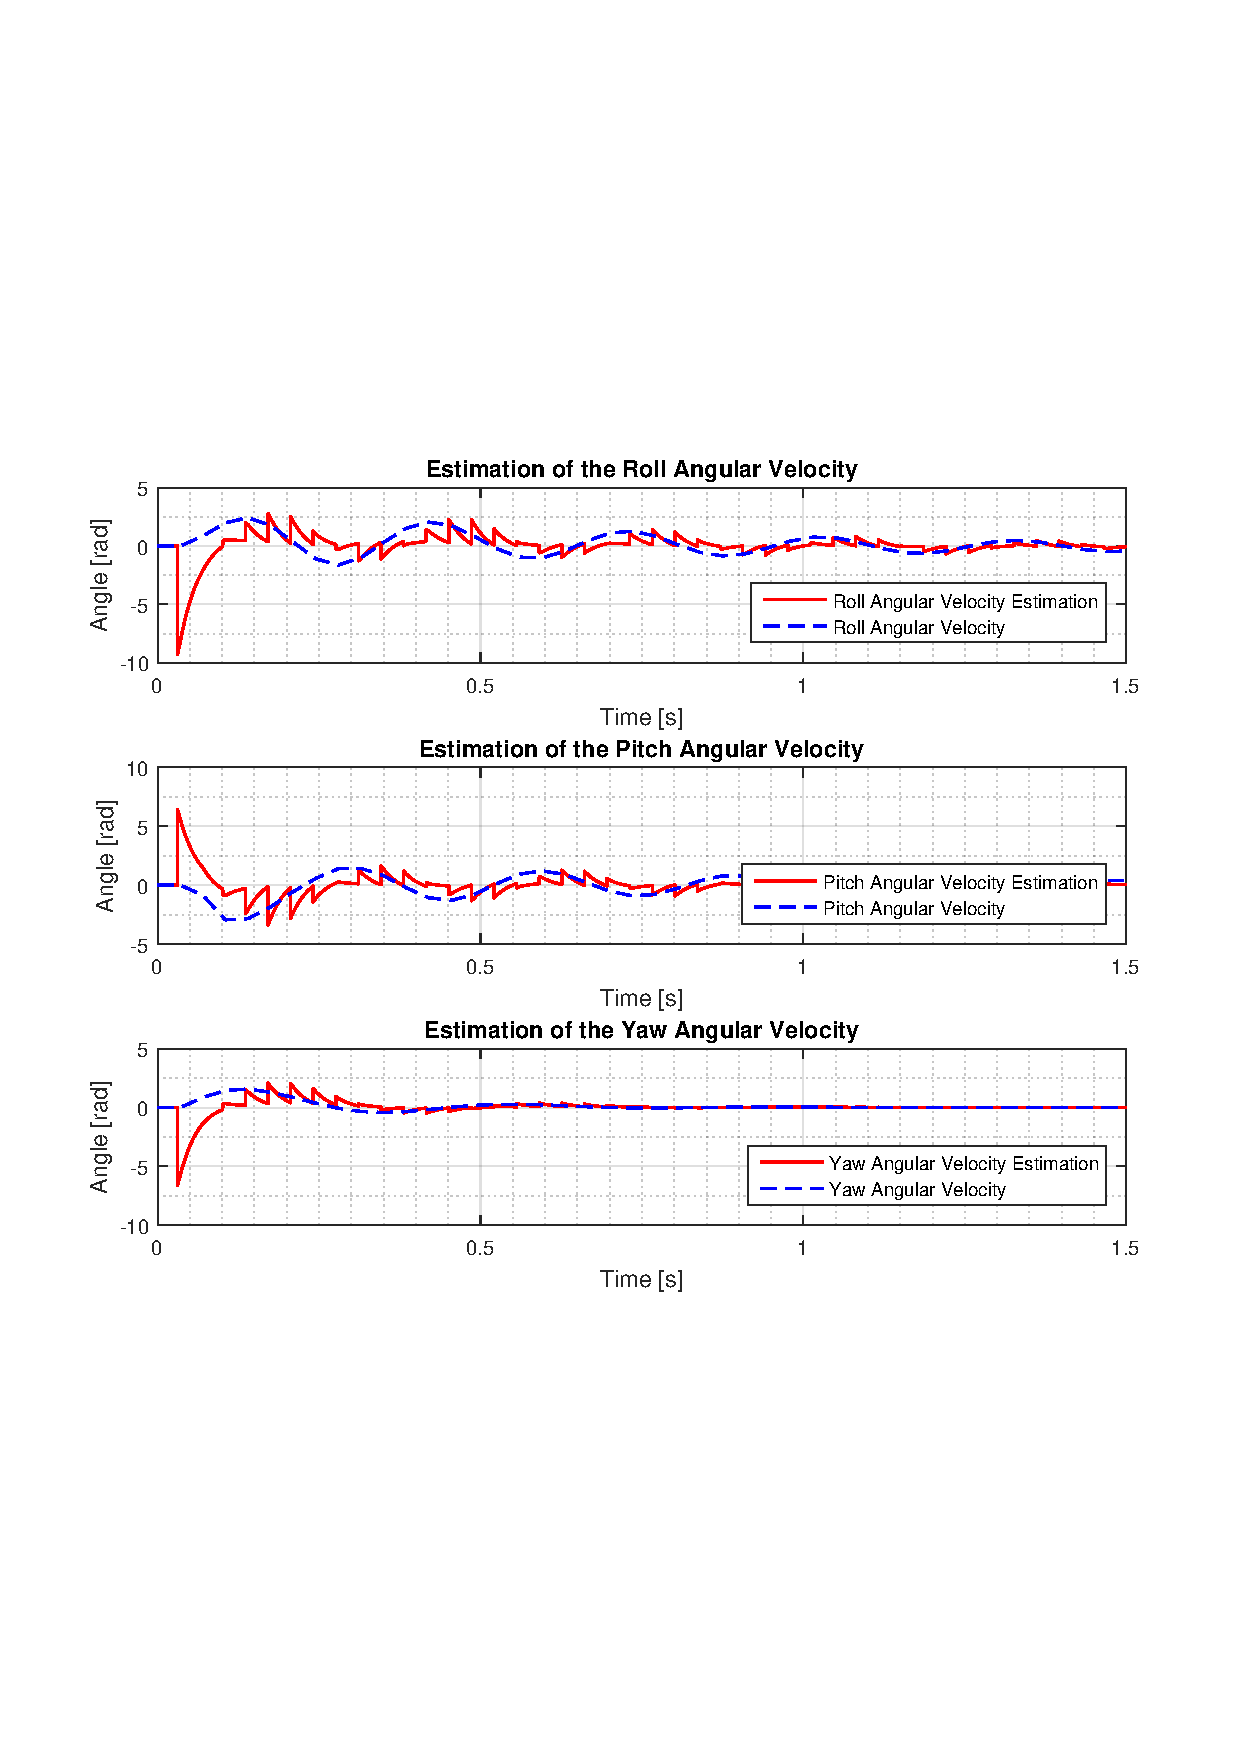
\includegraphics[scale=0.8]{figures/ssObsHigh.pdf}
	\caption{\autoref{app:matricesSS}.}
	\label{fig:TranslationalControlDiagram}
\end{figure}

Response with High observer L:

\begin{figure}[H]
	\centering
	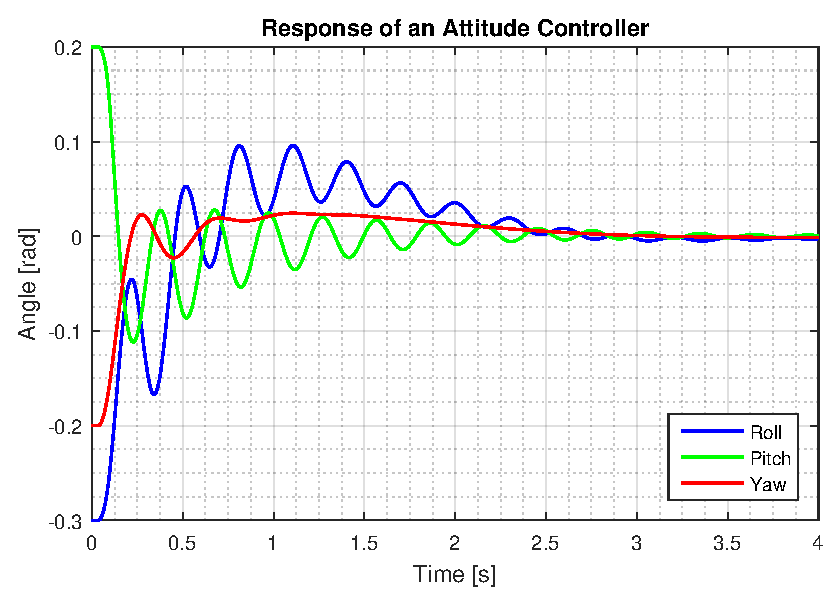
\includegraphics[scale=0.8]{figures/ssEqObsHigh.pdf}
	\caption{\autoref{app:matricesSS}.}
	\label{fig:TranslationalControlDiagram}
\end{figure}
